\documentclass{article}
\usepackage[utf8]{inputenc}
\usepackage{tikz}
\usepackage{graphicx}
\usetikzlibrary{arrows,positioning} 
\tikzset{
    %Define standard arrow tip
    >=stealth',
    %Define style for boxes
    punkt/.style={
           rectangle,
           rounded corners,
           draw=black, very thick,
           text width=6.5em,
           minimum height=2em,
           text centered},
    % Define arrow style
    pil/.style={
           ->,
           thick,
           shorten <=2pt,
           shorten >=2pt,}
}

\title{MOGPL - Projet 2015-2016}
\author{Jordi Bertran de Balanda}
\date{01/12/2015}

\begin{document}

\maketitle
\begin{abstract}
Nous modélisons et résolvons ici un problème de plus court chemin prenant en compte des couts de déplacement qui sont, à l'itération $n$, fonction de l'orientation de l'agent devant se déplacer dans la grille du problème à l'itération $n-1$.
\end{abstract}
\section{Modélisation et résolution du problème}
\subsection{Problème}
Le problème se présente comme un problème de plus court chemin dans un monde décrit par une grille de taille $M*N$ dont les chemins sont les sommets des cases de la grille. Le robot doit se mouvoir le long de ces chemins soit en tournant à gauche ou à droite ($TOURNE(x)$, x la direction), soit en avançant de 1, 2 ou 3 pas ($AVANCE(x), x \in {1, 2, 3}$).
Le problème définit une case de départ orientée, et une case d'arrivée sans contrainte d'orientation. La solution attendue est la suite de mouvements $TOURNE(x)$ et $AVANCE(x)$ de cout minimum, le cout étant de 1 par mouvement $TOURNE$ et de 1 par mouvement $AVANCE$, quel que soit le nombre de pas effectué.
\subsection{Modélisation}
Le problème posé peut aisément se modéliser comme un graphe orienté. Le fichier de données représentant le contenu des cases et non directement l'accessibilité des intersections des rails au robot, il est nécessaire d'effectuer une première passe sur les données pour obtenir une matrice représentant l'accessibilité de taille $(M+1)*(N+1)$.

On peut ensuite interpréter cette grille d'accessibilité comme un graphe orienté classique. Pour toute intersection de rails, il est possible d'atteindre les intersections situées 1, 2 ou 3 pas plus loin pour les 4 points cardinaux, avec un cout respectif de 1 pour la meme direction que celle avec laquelle l'intersection a été atteinte, 2 pour les directions orthogonales à celle-ci, et finalement de 3 pour la direction inverse.

\begin{figure}
\centering
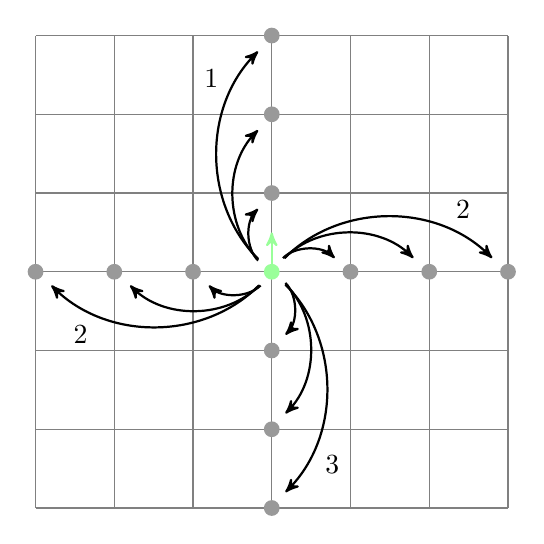
\begin{tikzpicture}[node distance=1cm, auto,]
\draw[step=1cm,gray,thin] (-3,-3) grid (3,3);
\node (robot) {};
\node[above=0.6cm of robot] (1a) {};
\node[above=1.6cm of robot] (2a) {};
\node[above=2.6cm of robot] (3a) {};
\node[left=0.6cm of robot] (1l) {};
\node[left=1.6cm of robot] (2l) {};
\node[left=2.6cm of robot] (3l) {};
\node[right=0.6cm of robot] (1r) {};
\node[right=1.6cm of robot] (2r) {};
\node[right=2.6cm of robot] (3r) {};
\node[below=0.6cm of robot] (1b) {};
\node[below=1.6cm of robot] (2b) {};
\node[below=2.6cm of robot] (3b) {};


\node (dummy) {} edge[pil, bend left=45] (1a.west) 
    edge[pil, bend left=45] (2a.west)
    edge[pil, bend left=45] node[near end] {1} (3a.west)
    edge[pil, bend left=45] (1r.north)
    edge[pil, bend left=45] (2r.north)
    edge[pil, bend left=45] node[near end] {2} (3r.north)
    edge[pil, bend left=45] (1b.east)
    edge[pil, bend left=45] (2b.east)
    edge[pil, bend left=45] node[near end] {3} (3b.east)
    edge[pil, bend left=45] (1l.south)
    edge[pil, bend left=45] (2l.south)
    edge[pil, bend left=45] node[near end] {2} (3l.south);
\fill[green!40!white] (0,0) circle (0.1cm);
\draw[thick,->, green!40!white] (0,0) -- (0,0.5);
\fill[black!40!white] (0,1) circle (0.1cm);
\fill[black!40!white] (0,2) circle (0.1cm);
\fill[black!40!white] (0,3) circle (0.1cm);
\fill[black!40!white] (1,0) circle (0.1cm);
\fill[black!40!white] (2,0) circle (0.1cm);
\fill[black!40!white] (3,0) circle (0.1cm);
\fill[black!40!white] (-1,0) circle (0.1cm);
\fill[black!40!white] (-2,0) circle (0.1cm);
\fill[black!40!white] (-3,0) circle (0.1cm);
\fill[black!40!white] (0,-1) circle (0.1cm);
\fill[black!40!white] (0,-2) circle (0.1cm);
\fill[black!40!white] (0,-3) circle (0.1cm);
\end{tikzpicture}
\caption{Accessibilité et couts à partir d'une intersection}
\label{fig:my_label}
\end{figure}

Afin de simplifier le suivi des directions prises et le calcul des couts correspondants, il est aisé de voir chaque intersection de rails comme un noeud quaternaire dans un graphe orienté, avec chaque noeud possédant une composante Nord, Sud, Est et Ouest. Ainsi, on peut facilement modéliser la différence de cout d'atteinte d'une intersection selon l'orientation du robot en arrivant à cette intersection, ce qui permet de calculer de manière immédiate les couts des voisins.

Après avoir pris en compte les contraintes de cout en fonction de l'orientation, le problème du robot se réduit donc à un problème de plus court chemin dans le graphe orienté possédant {4.M.N} noeuds. L'algorithme de Dijkstra est parfaitement adapté à ce problème, et sera utilisé pour le résoudre. En effet, le graphe n'est pas sans circuit puisque chaque noeud a la possibilité d'atteindre des noeuds prédécesseurs, et on ne peut donc pas utiliser l'algorithme de Bellman-Ford.

\subsection{Résolution}
La résolution du problème se déroule en 3 étapes.

La première étape est de transformer la matrice fournie en entrée en matrice de noeuds accessibles/inaccessibles pour le robot. Ceci se fait en $M*N$ itérations, avec l'interrogation d'au plus 4 cases de la matrice en entrée pour déterminer si le noeud de coordonnées correspondantes de la matrice des rails est accessible. S'il est accessible, la case de la matrice des rails devient un dictionnaire de 4 noeuds représentant les 4 états possibles du robot lorsqu'il atteint le noeud: Nord, Sud, Est et Ouest.

La deuxième étape est le déroulement de l'algorithme de Dijkstra. Les voisins éventuels du noeud traité, au nombre d'au plus 12 comme indiqués sur la figure 1, sont obtenus à la volée en regardant la matrice des rails au lieu d'etre stockés dans une liste pour chaque noeud. La liste des voisins non traités est gérée par un tas minimum, qui permet de suivre la valeur minimale des couts locaux avec une complexité très faible. L'algorithme s'arrete une fois que les 4 noeuds correspondant aux coordonnées définies par l'objectif ont été marqué comme entièrement traités, ou quand la liste de voisins à traiter devient vide.

La troisième étape est de remonter à partir du noeud de cout minimum parmi les noeuds de coordonnées correspondantes à l'objectif. Jusqu'à obtenir le noeud de départ, on examine la différence de position entre le noeud courant et son parent optimal, et on en extrapole les mouvements à effectuer pour atteindre le noeud courant à partir du parent. Ce mouvement est au plus constitué de deux instruction $TOURNE$ et d'une instruction $AVANCE$. Cette suite d'instruction, associée au cout minimum dans les noeuds objectifs, produit la solution à l'instance du problème.

\section{Code}
Le code rendu est écrit en Python. Il utilise les librairies heapq pour pouvoir suivre le minimum d'une liste à faible cout, matplotlib pour la production des graphiques d'évaluation de performances, et sys/os pour des fonctions d'entrée/sortie. La logique se trouve dans problem.py, les outils divers dans tools.py.
L'interface graphique est codée en utilisant le binding Python pour la bibliothèque QT4. La logique de l'interface se trouve dans robot.py, et la description de l'interface dans gui.py.
\subsection{Classes importantes}
\subsubsection{Problem}
La classe Problem contient toutes les informations nécéssaires à la description d'un problème, ainsi que la logique haut niveau nécessaire à sa résolution. Elle déclenche des opérations sur les classes Node et RailMatrix contenant la logique fine de résolution du problème (passe de transformation de la matrice, calculs d'accessibilité, mise à jour des voisins...). Elle contient également des opérations statiques pour la mise en forme de la solution
\subsubsection{RailMatrix}
La classe RailMatrix contient les informations utiles au déroulement de l'agorithme de Dijkstra: la grille de noeuds obtenue à l'étape 2 de la résolution du problème et le tas minimum servant à suivre les noeuds à traiter.
\subsubsection{Node}
La classe Node contient la logique de mise à jour des noeuds de la matrice de rails essentielle au déroulement de l'algorithme.
L'exécution des méthodes d'évaluation de performances entraine également la production des fichiers correspondant aux problèmes aléatoires générés dans le dossier FichiersPb.
\subsection{Utilisation}
\begin{verbatim}
python projet.py -g
\end{verbatim}
Lance l'interface graphique.
\begin{verbatim}
python projet.py -f mesFichiers
\end{verbatim}
Délenche la lecture et la résolution des instances de problème contenues dans mesFichiers
\begin{verbatim}
python projet.py -test
\end{verbatim}
Exécute une batterie de tests de fonctions (lecture, écriture, génération aléatoire, résolution...)
\begin{verbatim}
python projet.py -testSize
\end{verbatim}
Génère et résout des instances aléatoires de tailles différentes, puis affiche un graphe résumant les temps d'exécution.
Consigne les problèmes et leurs solutions dans des fichiers correspondants dans ./FichiersPb.
\begin{verbatim}
python projet.py -testObs
\end{verbatim}
Génère et résout des instances aléatoires de taille 20*20 avec des nombres d'obstacles différents, puis affiche un graphe résumant les temps d'exécution.
Consigne les problèmes et leurs solutions dans des fichiers correspondants dans ./FichiersPb.
\section{Performances}
\subsection{En fonction de la taille du problème}
\begin{figure}[!ht]
\centering
\includegraphics[scale=0.6]{sizeFig.png}
\caption{Temps moyens de résolution de problèmes aléatoires en fonction de leur taille (10 instances par taille)}
\end{figure}
En considérant une matrice problème sans obstacles, l'algorithme considère au plus $NM$ noeuds quaternaires, soit au plus $4NM$ noeuds à traiter lors de la résolution. Ainsi, on s'attend, dans une matrice carrée, à une courbe de temps de résolution quadratique en fonction de la taille de la matrice. 
\subsection{En fonction du nombre d'obstacles}
Lors de la résolution, on considère dans une matrice $20*20$ sans obstacles $1600$ noeuds. Chaque obstacle rajouté retire $4$ noeuds. On résoud donc le problème dans un graphe de $1600 - 4*o$ noeuds, avec $o$ le nombre d'obstacles. On s'attend donc à constater que le temps de résolution diminue en fonction du nombre d'obstacles, puisqu'à chaque obstacle ajouté on restreint le nombre de noeuds à traiter pour terminer l'algorithme.
\begin{figure}[!ht]
\centering
\includegraphics[scale=0.6]{obsFig.png}
\caption{Temps moyens de résolution de problèmes aléatoires de taille 20x20 en fonction du nombre d'obstacles (10 instances par nombre d'obstacles)}
\end{figure}
\end{document}
